
\section{Second raffinement}


%\subsection{}
%\paragraph{}

\subsection{Analyse}
On introduit dans ce dernier raffinement les autorisations d'accès à la piste et les identifiants uniques à chaque avions. Un pilote effectue une demande d'accès
à la piste. Le système répond en accordant ou refusant le droit d'accès. 

\begin{itemize}
	\item Si l'accès est accordé, le pilote a 15 mn pour libérer la piste.
	\item S'il est refusé, le pilote doit attendre 5 mn avant de pouvoir renouveler sa demande.   
\end{itemize}  

\subsection{Contexte}
On étend le contexte0 précédent avec le contexte2

\begin{figure}[H]
	\begin{center}	
		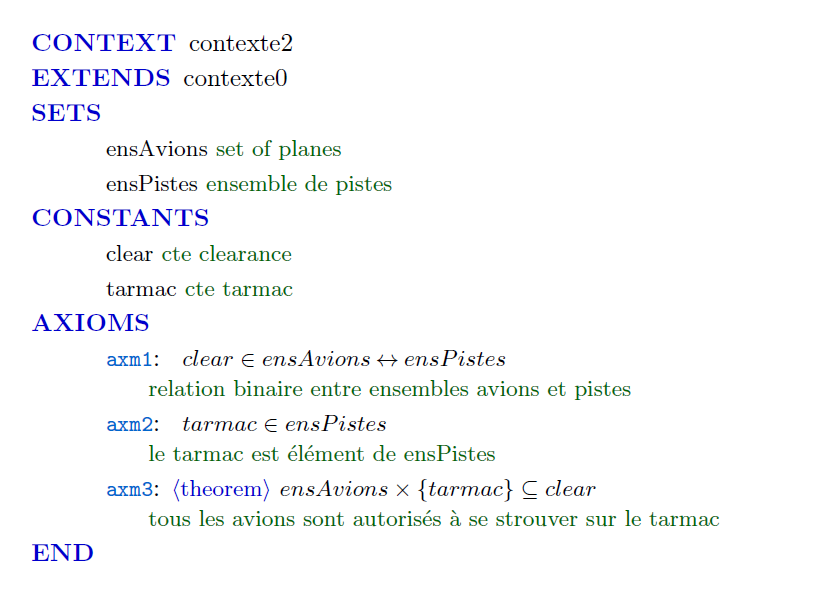
\includegraphics[scale=0.7]{images/2/ctx2}
		\caption{Contexte second raffinement}
		\label{ctx2}
	\end{center}
\end{figure}

\subsection{Glue} 
Le lien avec la machine raffinement1 est réalisé par le biais du nombre d'avions respectivement sur le tarmac, la piste décollage et la piste d'atterrissage. Une approche ensembliste, analogue à celle utilisée dans un système de contrôle d'accès à des bâtiments d'un site, conduit à introduire les ensembles d'avions correspondant. Les invariants de cardinalité, inv 16, 17 et 18 de la figure \ref{raf21} assure la liaison avec la machine parente. 


On crée une nouvelle machine nommée raffinement2 comme ci-après. Les commentaires ont été directement saisis dans l'interface rodin. Les livrables sont accessibles
en ligne via l'URI \url{https://github.com/kad15/eventb/tree/master/LIVRABLE_HELLER_BELDJILALI/workspace_rodin}.
\begin{figure}[H]
	\begin{center}	
		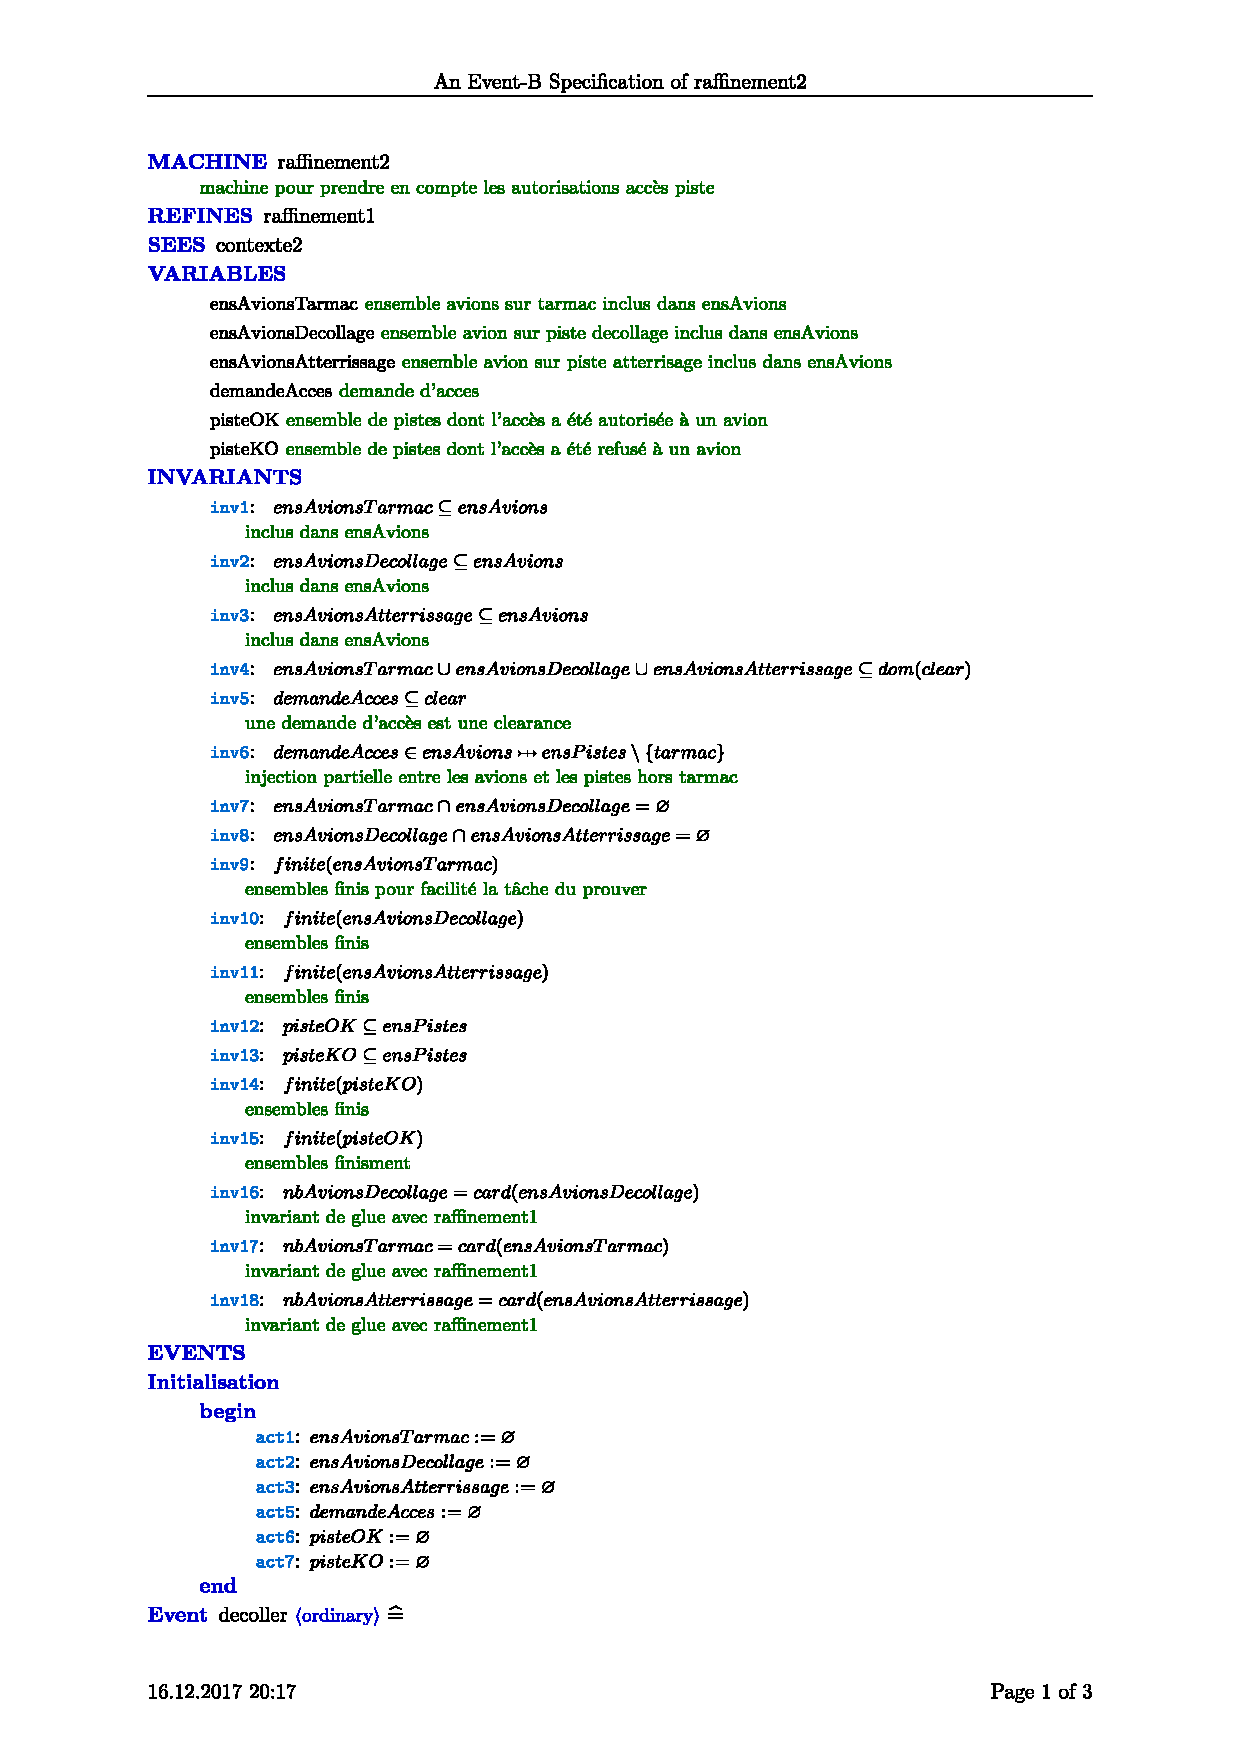
\includegraphics[scale=0.75]{images/2/raf21.pdf}
		\caption{ Machine : second raffinement}
		\label{raf21}
	\end{center}
\end{figure}

\begin{figure}[H]
	\begin{center}	
	
		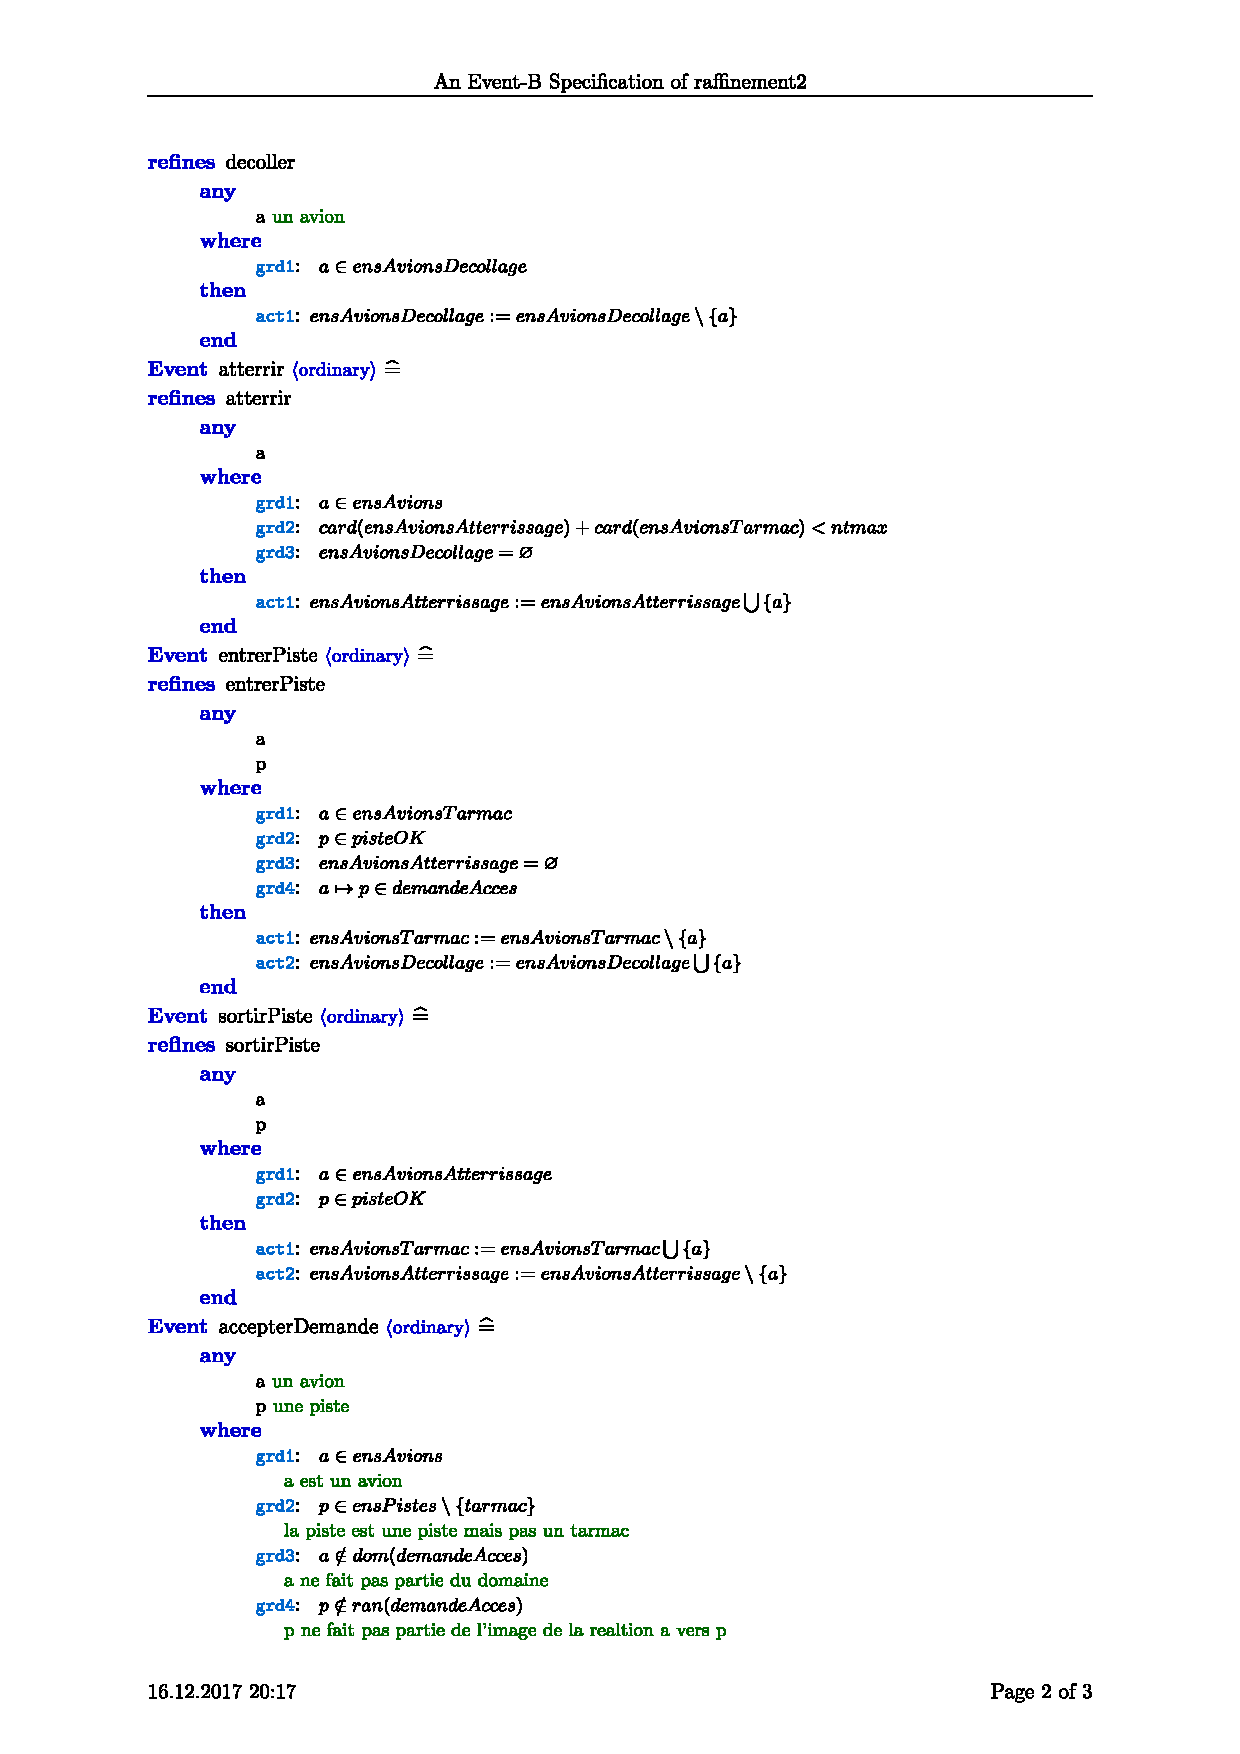
\includegraphics[scale=0.75]{images/2/raf22.pdf}
		\caption{ Machine : second raffinement (suite)}
		\label{raf22}
	\end{center}
\end{figure}


\begin{figure}[H]
	\begin{center}	
		
		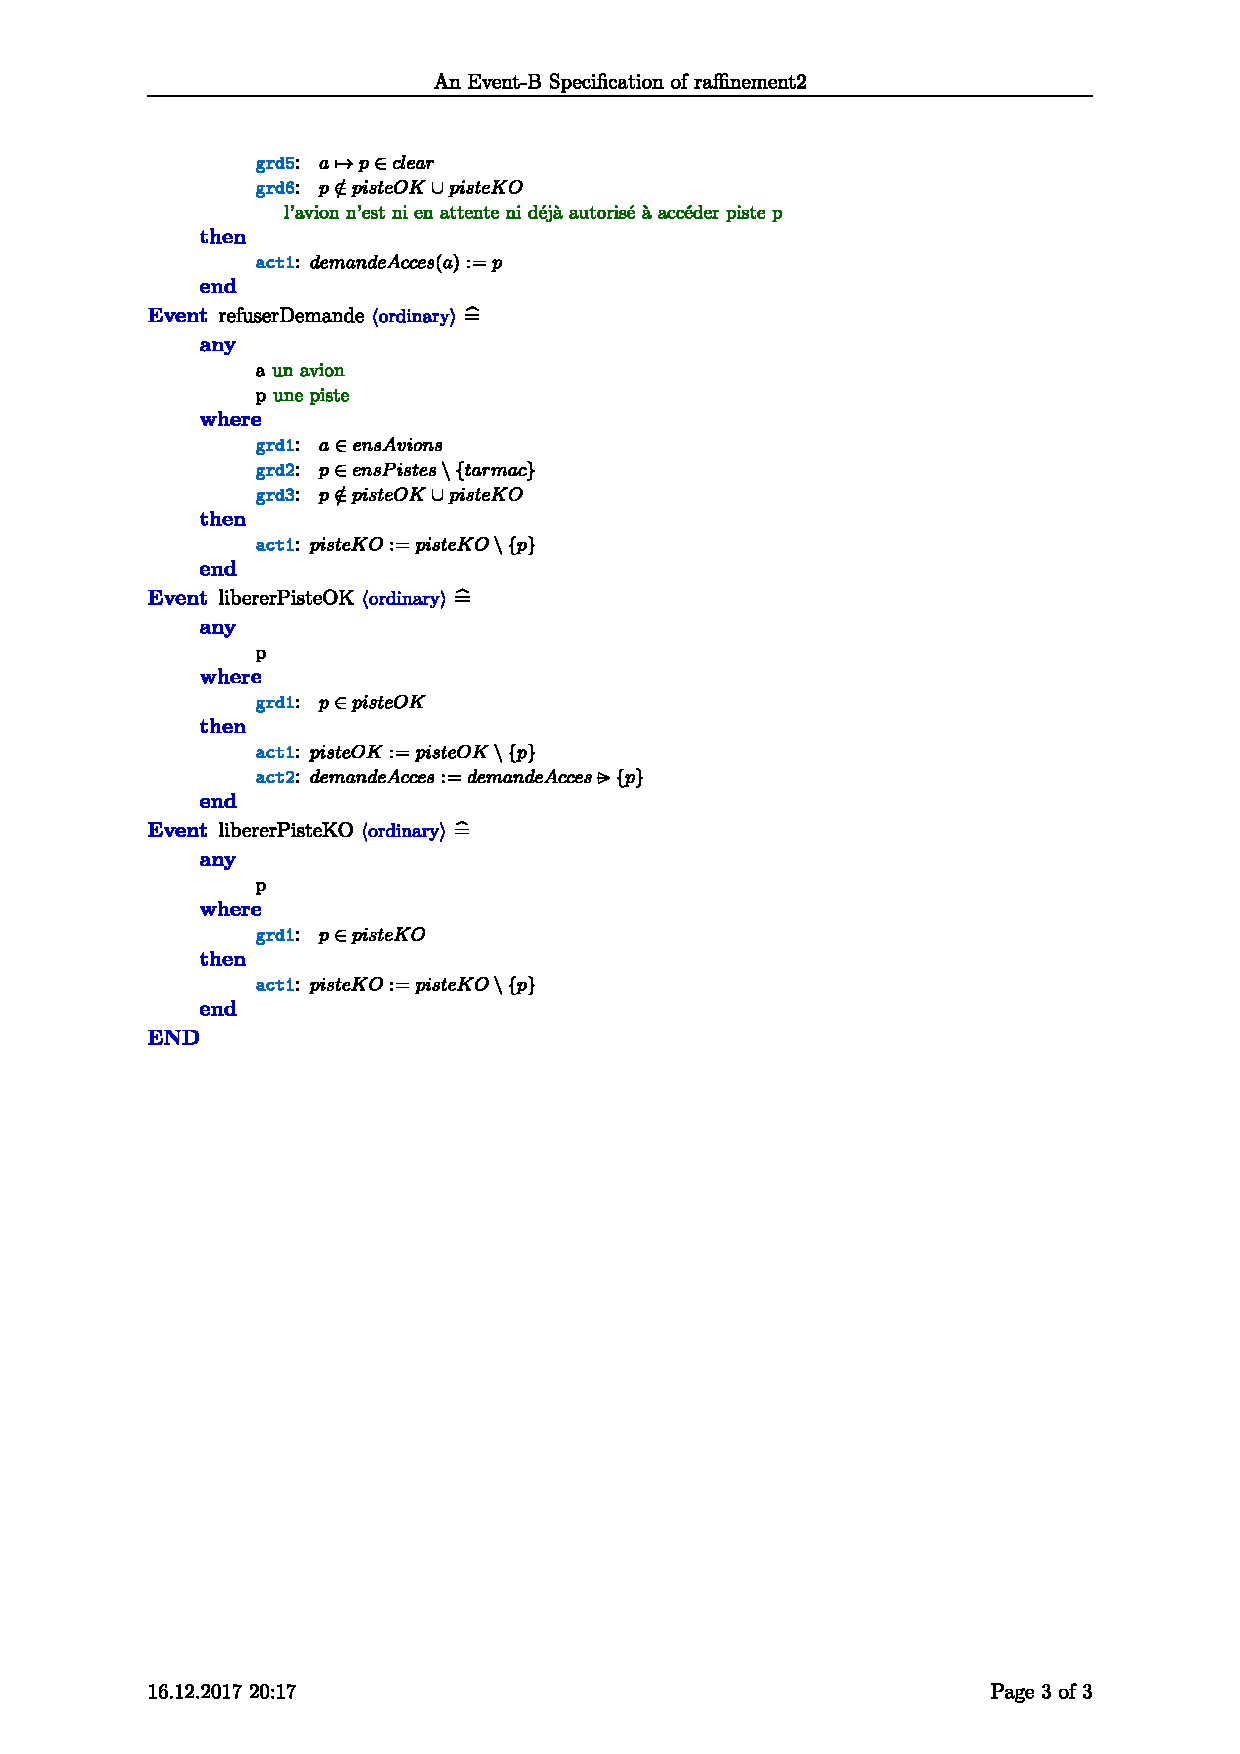
\includegraphics[scale=0.75]{images/2/raf23.pdf}
		\caption{ Machine : second raffinement (suite)}
		\label{raf23}
	\end{center}
\end{figure}


\subsection{Preuves}


\begin{figure}[H]
	\begin{center}	
		
		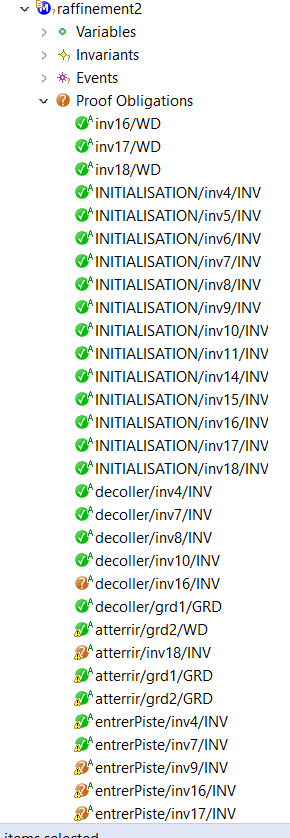
\includegraphics[scale=0.75]{images/2/proof2}
		\caption{ Résultat des preuves des propriétés générées par l'outil rodin - atelier B}
		\label{proof 2}
	\end{center}
\end{figure}

On constate que le système n'est pas entièrement validé. En outre, l'outil rodin indique une syntaxe incorrecte pour l'instruction $ensAvionsTarmac := ensAvionsTarmac ⋃ \{a\}$ alors qu'elle semble correcte.


